% command to make sure colorboxes don't create whitespace between code lines
\fboxsep=.6pt

% default settings for listings
\lstset{style=python}

\title[Programmieren]{Programmieren: Verzweigungen}

\subtitle{Konditionale Schleifen-Abbrüche mit \lstinline|while| und \lstinline|break|}

\author[Blum, Cyril] % (optional)
{Cyril Blum}

\institute[KLW] % (optional)
{
    Fachschaft Informatik\\
    Kantonsschule im Lee
}

\date[\today] % (optional)

\logo{
\includegraphics[width=2cm]{Logos/LeeLogo}}

\titlegraphic{\vspace{-.7cm}\includegraphics[width=\textwidth]{"Grundlagen_Info/06_Datenbanken/Figures/title-emojis"}}

\frame{\titlepage}

\begin{frame}[fragile]{Spirale: Abbruchkondition?}
    \begin{columns}
        \begin{column}{.7\textwidth}
            \begin{lstlisting}
import turtle as t

def spirale(seite, add, max_seite):
    for _ in range(?):
        t.fd(seite)
        t.rt(90)
        seite+=add

spirale(10, 10, 100)
\end{lstlisting}
            Wie viele Male muss das \lstinline|for _ in range(?)| ausgeführt werden?
            \only<2->{
                \[\floor{\frac{\text{\texttt{maxseite - seite}}}{\text{\texttt{add}}}} + 1\]
            }
            \only<3->{
                Es geht auch einfacher $\ldots$
            }
            
        \end{column}

        \begin{column}{.3\textwidth}
            \begin{figure}
                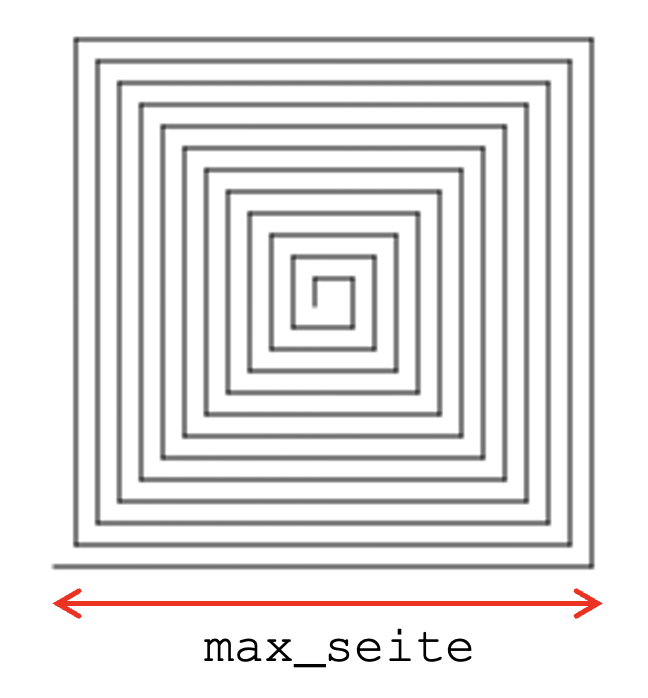
\includegraphics[width=\linewidth]{Grundlagen_Info/00_Programmieren/Figures/spirale_while}
            \end{figure}
        \end{column}
    \end{columns}
\end{frame}

\begin{frame}[fragile]{Spirale: Flussgesteuerter Abbruch (\lstinline[basicstyle=\ttfamily]|break|)}
    \begin{columns}
        \begin{column}{.7\textwidth}
            \begin{lstlisting}[escapechar=!]
import turtle as t

def spirale(seite, add, max_seite):
    while True:!\tikzmark{repeatFrom}!       !\tikzmark{repeat}!
    	if seite > max_seite:
    	    break!\tikzmark{breakFrom}!         !\tikzmark{break}!
        t.fd(seite)
        t.rt(90)
        seite+=add

spirale(10, 10, 100)
\end{lstlisting}
        \end{column}
        \begin{column}{.3\textwidth}
            \begin{figure}
                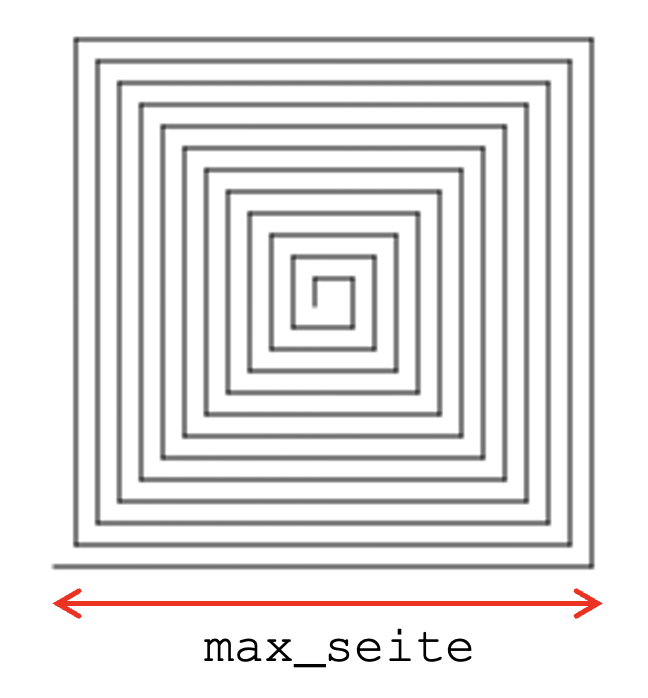
\includegraphics[width=\linewidth]{Grundlagen_Info/00_Programmieren/Figures/spirale_while}
            \end{figure}
        \end{column}
    \end{columns}

    \begin{tikzpicture}[overlay, remember picture,
            every node/.style={draw=red!50,fill=red!50!white,text=black,rounded corners}]
        \drawArrow{repeatFrom}{repeat}{\footnotesize Endlosschleife}{CarnationPink};
        \drawArrow{breakFrom}{break}{\footnotesize Schleifenabbruch}{CarnationPink};
    \end{tikzpicture}

\end{frame}

\begin{frame}[fragile]{Fuss- und kopfgesteuerte Schleifen}
    \begin{columns}
        \begin{column}{.47\textwidth}
            \begin{lstlisting}[escapechar=!,basicstyle=\footnotesize\ttfamily]
import turtle as t

def spirale(seite, add, maxS):
    while True:            !\tikzmark{fromStart}!
    	if seite > maxS:
    	    break          !\tikzmark{fromEnd}!
        t.fd(seite)
        t.rt(90)
        seite+=add

spirale(10, 10, 100)
\end{lstlisting}
        \end{column}
        \begin{column}{.5\textwidth}
            \begin{lstlisting}[escapechar=!,basicstyle=\footnotesize\ttfamily]
import turtle as t

def spirale(seite, add, maxS):
    !\tikzmark{toStart}!!\tikzmark{toEnd}!while seite < maxS:
        t.fd(seite)
        t.rt(90)
        seite+=add
        
spirale(10, 10, 100)
\end{lstlisting}
        \end{column}
    \end{columns}

    % annotate listings
    \begin{tikzpicture}[overlay, remember picture,
            every edge/.append style = { ->, thick, >=stealth, red!70},
            every node/.style={draw=red!50,fill=red!50!white,text=black,rounded corners}]
        \only<2->{
            \drawBrace{0em}{fromStart}{fromEnd}{}{.5}{}{}
		    \drawBrace{-.5em}{toStart}{toEnd}{}{.5}{mirror}{}
            % arrow pointing from one code to other
            \draw[->, style={thick, >=stealth, red!70}] (fromStartfromEnd-coord-arrow) to (toStarttoEnd-coord-arrow);
        }
    \end{tikzpicture}
\end{frame}

\begin{frame}[fragile]{Wichtige Bemerkungen}
    \begin{itemize}[<+->]
        \item \lstinline|break| bricht nicht aus \lstinline|def| aus, sondern aus der (aktuellen) \lstinline|while True|-Schleife!
        \item Ein \lstinline|while True:| (unendliche Schleife) ohne \lstinline|break| kann zum Absturz des Programms führen \emoji{face-with-spiral-eyes}
        \item Je nachdem kann das auch in einem \lstinline|while| passieren, sofern die Bedingung nach dem \lstinline|while| so geschrieben ist, dass sie immer wahr (\lstinline|True|) ist.
        \item \textbf{Speichern Sie regelmässig Ihre Aufgaben!}
        \item Falls das Programm endlos weiterläuft: Python beenden \faTrash
    \end{itemize}
\end{frame}

\begin{frame}[fragile]{Aufträge}
    \begin{itemize}
        \item \lstinline|break|
        \begin{itemize}
             \item \aufgabebox{Aufgaben 5.24 - 5.26}
            \item \challengebox{Aufgabe 5.27}
        \end{itemize}
        \item \lstinline|while| mit Bedingung:
        \begin{itemize}
             \item \aufgabebox{Aufgaben 5.28 - 5.35}
        \end{itemize}
    \end{itemize}
\end{frame}
